%----------------------------------------------------------------------------------------
%	PACKAGES AND OTHER DOCUMENT CONFIGURATIONS
%----------------------------------------------------------------------------------------

\documentclass[12pt]{article}
\usepackage[danish]{babel}
\usepackage{mathtools}
\usepackage[euler]{textgreek}
\usepackage[numbered,final]{mcode}
\usepackage[utf8x]{inputenc}
\usepackage{amsmath}
\usepackage{graphicx}
\usepackage[colorinlistoftodos]{todonotes}
\usepackage[toc,page]{appendix}
%\usepackage{float}
\usepackage{floatrow} % used for adding "Source" to pictures
\usepackage{hyperref} % used for hyperlinks
\usepackage[all]{hypcap}
\usepackage{bm} % used for bold inline matj
\usepackage{lipsum} % used for lorem lipsum
\usepackage[final]{pdfpages} % used for including PDF's
\usepackage{geometry}
\usepackage{listingsutf8}
\usepackage{listings}
\usepackage{blindtext}
\usepackage{enumitem}
\usepackage{color} %red, green, blue, yellow, cyan, magenta, black, white
\definecolor{mygreen}{RGB}{28,172,0} % color values Red, Green, Blue
\definecolor{mylilas}{RGB}{170,55,241}
\hypersetup{colorlinks=true, linkcolor=black}

% Page margins
\geometry{verbose,tmargin=1in,bmargin=1in,lmargin=1in,rmargin=1in,headsep=0.35in}

\begin{document}
	
	\begin{titlepage}
		
		
		
		\newcommand{\HRule}{\rule{\linewidth}{0.5mm}} % Defines a new command for the horizontal lines, change thickness here
		\setlength{\topmargin}{0in}
		\centering % Center everything on the page
		
		%----------------------------------------------------------------------------------------
		%	HEADING SECTIONS
		%----------------------------------------------------------------------------------------
		\textsc{\LARGE Aarhus universitet}\\[1.5cm] % Name of your university/college
		\textsc{\Large Anvendte microcontroller systemer}\\[0.5cm] % Major heading such as course name
		\textsc{\large 6. Semester}\\[0.5cm] % Minor heading such as course title
		
		%----------------------------------------------------------------------------------------
		%	TITLE SECTION
		%----------------------------------------------------------------------------------------
		
		\HRule \\[0.4cm]
		{ \huge \bfseries Color Sorting System}\\ % Title of your document
		\HRule \\[1cm]
		
		%----------------------------------------------------------------------------------------
		%	AUTHOR SECTION
		%----------------------------------------------------------------------------------------
		
		\begin{minipage}{0.4\textwidth}
			\begin{flushleft} \large
				\emph{Gruppemedlemmer:}\\
				Daniel Tøttrup \\
				Stinus Lykke Skovgaard \\
			\end{flushleft}
		\end{minipage}
		~
		\begin{minipage}{0.4\textwidth}
			\begin{flushright} \large
				\emph{AUID} \\
				au544366\\
				au520659\
			\end{flushright}
		\end{minipage}\\[5cm]
		
		%----------------------------------------------------------------------------------------
		%	LOGO SECTION
		%----------------------------------------------------------------------------------------
		
		
\includegraphics[scale=0.5]{Img/logo.jpg}\\[1cm]
		
		%----------------------------------------------------------------------------------------
		%	DATE SECTION
		%----------------------------------------------------------------------------------------
		
		{\large \today}\\[0.5cm] % Date, change the \today to a set date if you want to be precise
		
		
		\vfill % Fill the rest of the page with whitespace
		
	\end{titlepage}
	
\newpage
\tableofcontents
\newpage
\listoffigures
\newpage

\hypersetup{linkcolor=blue}



%!TEX root = ../../Main.tex
\graphicspath{{Chapters/Indledning/}}
%-------------------------------------------------------------------------------

\section{Indledning}


\begin{figure}[H]
	\centering
	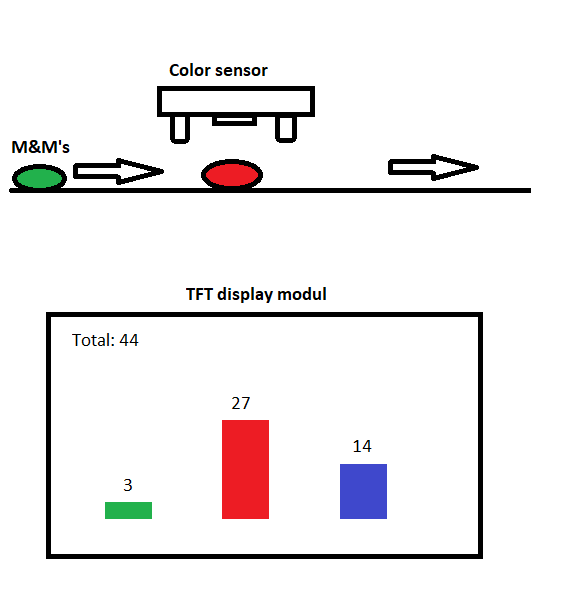
\includegraphics[width = 400pt]{Img/KonceptBillede}
	\caption{Konceptbillede for CSS}
	\label{fig:konceptbillede}
\end{figure}

Color Sorting System(CSS) gør det nemt at sortere diverse emner baseret på deres farve. Disse emner kan være alt fra fødevare til maskin-komponenter, så længe de kan identificeres på farve. CSS fungerer ved at lade emnet passere under en farve sensor, som kan identificere farven på emnet og videresende hvilken farve emnet har til et TFT displaymodul. På koncept billedet på \autoref{fig:konceptbillede}, kan man se at M\&M's bliver talt op hver gang de paserer sensoren. TFT modulet kan så ved hjælp af søjle diagrammer, fortælle hvor mange forskellige farvet emner der har passeret sensoreren. Resultaterne kan gemmes på et SD kort, hvis man senere skulle bruge dataen. Dog er implementeringen af SD kortet ikke fuldendt i denne prototype, og vil i en viderudvikling af projektet have stor prioritet. Desuden er der kun lagt vægt på color sensor og TFT display modulerne, hvilket vil sige at selve sorteringsmekanikken ikke er implementeret i den nuværende prototype.
	
\newpage


	%!TEX root = ../../Main.tex
\graphicspath{{Chapters/Krav/}}
%-------------------------------------------------------------------------------


\section{Krav}
I dette afsnit beskrives kravene til CSS og hvilken funktionalitet systemet skal have. Der er stillet nogle enkelte krav fra kursets side, hvor nogle af disse krav skal indgå i projektet:

\begin{itemize}
	\item Use In Circuit debug tools
	
	\item Implement Drivers, dealing with time critical parameters.
	
	\item Implement Boot Loaders for updating microcontroller firmware
	
	\item Use USB to interface a microcontroller
	
	\item Use operating systems for microcontrollers
	
	\item Use microcontroller knowledge in a final mini project
	
\end{itemize}

Flere af disse krav er implementeret i CSS. Der er brugt tidskritiske drivers til color sensoren, display modulet og til implementeringen af I2C mellem de to microcontrollers. 

\begin{figure}[H]
	\centering
	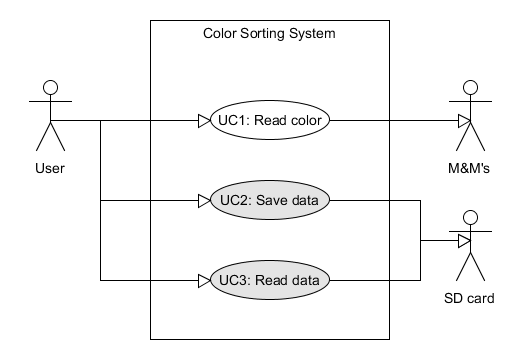
\includegraphics[width = 400pt]{Img/Usecase_diagram.png}
	\caption{Usecase diagram for CSS}
	\label{fig:UsecaseDiagram}
\end{figure}

På \autoref{fig:UsecaseDiagram} ses usecase diagrammet som beskriver sammenhængen mellem aktørerne og de forskellige funktionaliteter der findes for systemet. Uscase 2 og 3 er grå, hvilket betyder at de ikke er implementeret i prototypen. 

\subsection{UC1 - Read Color}
Denne usecase danner ramme for hvordan CSS måler en farve. Brugeren placerer emne der ønsket aflæst. Brugeren trykker på aflæs-knappen og den aflæste farve kan nu ses talt op på TFT display modulet.

\subsection{UC2 - Save Data}
Denne usecase danner ramme for, at gemme data på SD kort. Brugeren trykker på "Save Data" knappen på skærmen. Data bliver derefter gemt på SD kort.

\subsection{UC3 - Read Data}
Denne usecase danner ramme for, at hente data fra SD kortet. Brugeren trykker på "Load Data" knappen på skærmen. Gemt data bliver hentet fra SD kortet og vist på TFT skærmen.

\subsection{Afgrænsning}
Det skal sige at usecase 2 og 3 ikke er implementeret i denne protorype. Der er gjort forsøg på at få dem implementeret, men grundet tidspres blev de nedprioriteret. Derudover var det også tænkt fra start, at der ikke skulle være behov for brugerinput for at kunne aflæse farve, men på grund af tidsmangel fik gruppen ikke implementeret et system der kunne fodre CSS med emner. Dette gøres istedet for manuelt og vil i fremtiden skulle noget automatisering af CSS implementeres.


%!TEX root = ../../Main.tex
\graphicspath{{Chapters/Diskussion/}}
%-------------------------------------------------------------------------------


\section{Systemarkitektur}


Vores systemarkitektur fungerer som den overordnede ramme for hvordan vi senere har implementeret vores system. Dette afsnit vil give et overblik over vores systems arkitektur, for at give et overskueligt overblik over systemet. Det er her at den beskrevne funktionalitet deles ud i mindre moduler. 

\subsection{Blokidentifikation}
På figur \autoref{fig:ColorSortingSystem_BDD}  ses det overordnede BDD, som beskriver de enkelte moduler som systemet indeholder. Hver blok beskriver en funktionalitet, som systemet håndterer. I det følgende vil de enkelte moduler og funktionalitet kort beskrives.

\begin{figure}[H]
	\centering
	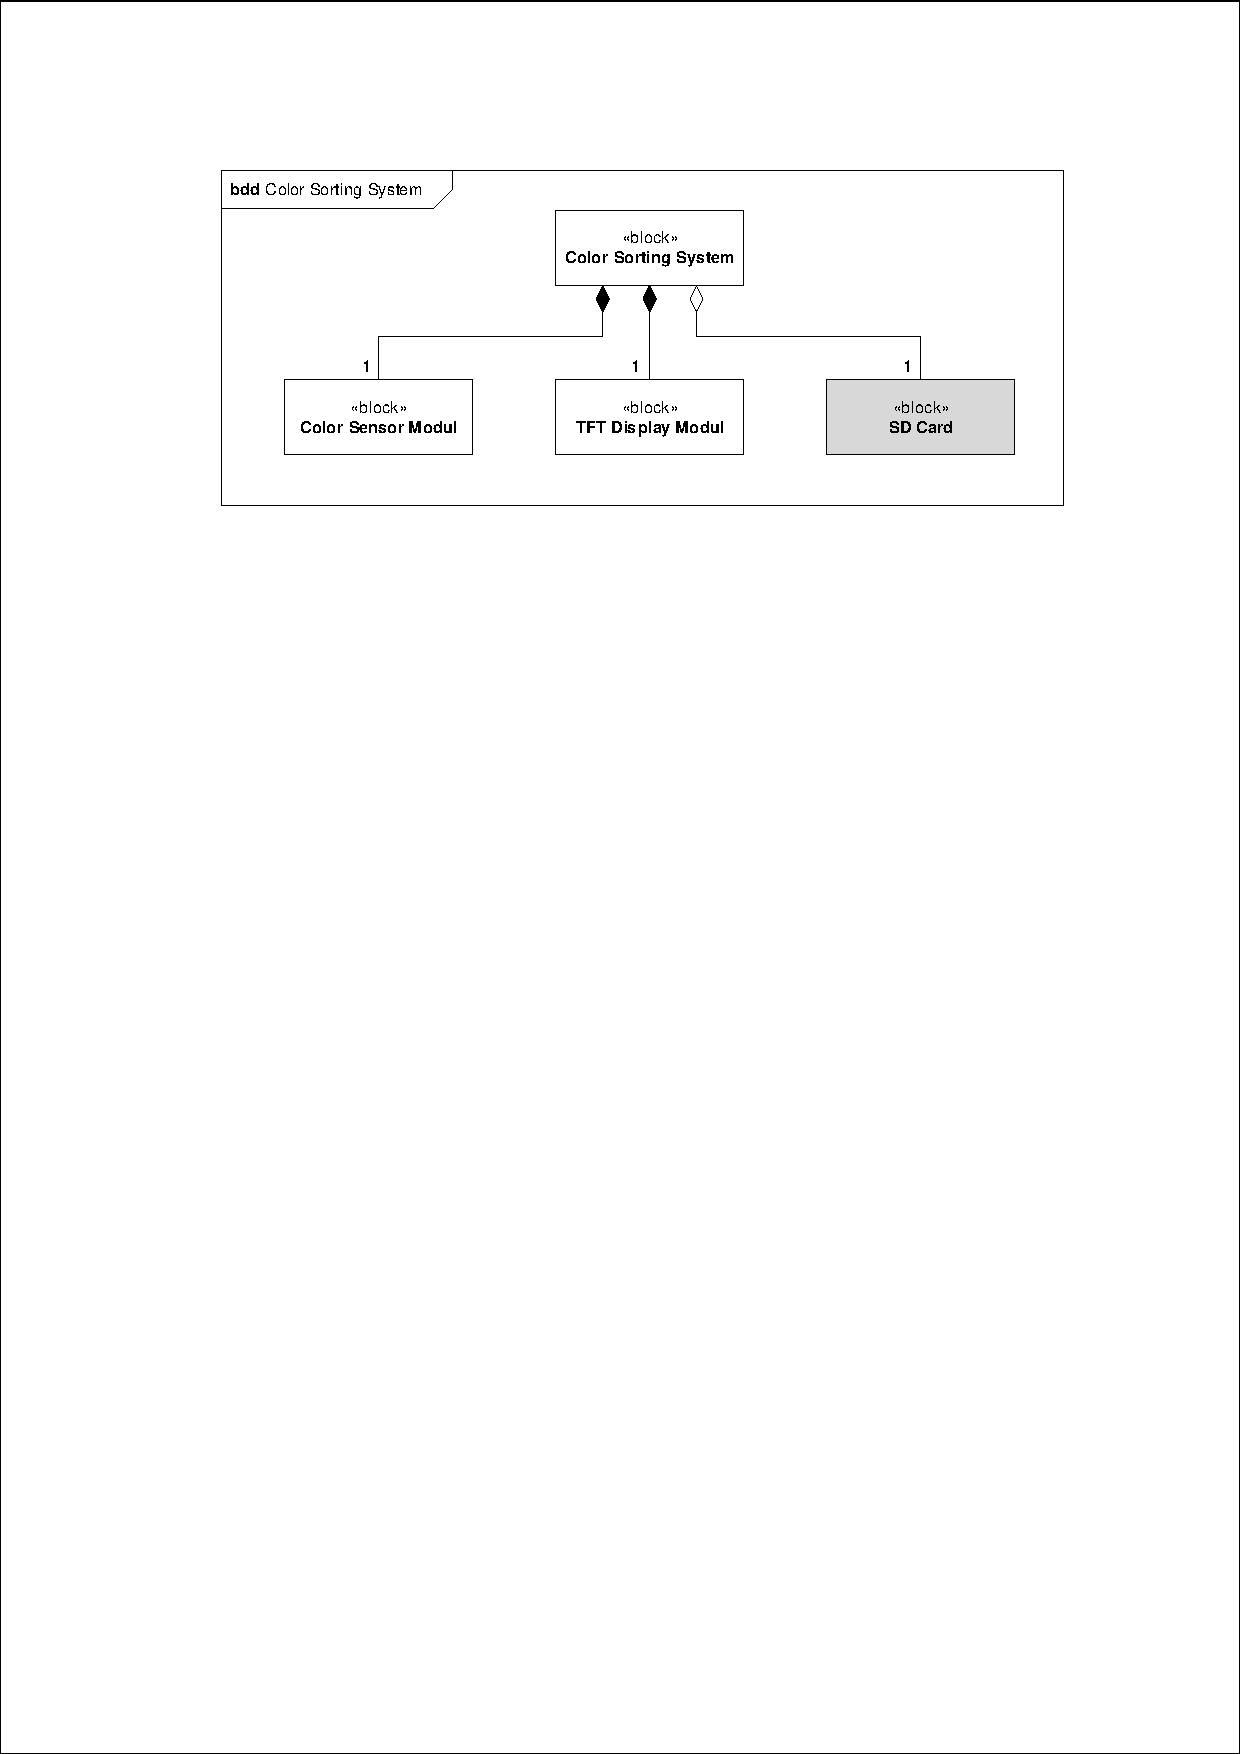
\includegraphics[width = 400pt]{Img/ColorSortingSystem_BDD.png}
	\caption{Color Sorting System BDD}
	\label{fig:ColorSortingSystem_BDD}
\end{figure}

\textbf{TFT Display Module:} \\
Har til opgave at modtage data fra Color Sensor Module og vise brugeren på baggrund af det modtaget data, antallet af hver enkelt farve målt, samt det totale antal farver. Dette modul skulle også havde haft ansvaret for at sende data til SD-kortet, hvis den del var blevet implementeret. 
\\\textbf{Color Sensor Module:} \\
Har til opgave at måle farven placeret under Color Sensoren, samt sende informationen videre til TFT Display Module.
\\\textbf{SD-Kort:}\\
Et SD kort som var tiltænkt at kunne opbevare data som efter systemet slukkes. Dette blev dog taget ud af system. Hvilket visualiseres ved den grå farve i BDD’et.  

\subsection{Blokinteraktion}

På \autoref{fig:ColorSortingSystem_IBD} nedenfor ses det overordnede IBD for systemet. IBD’et viser de forskellige hardwareblokke i systemet og deres interaktion mellem hinanden. Interaktionen mellem blokkene bliver beskrevet mere detaljeret under dokumentationen for de enkelte blokke. I forhold til det overordnede BDD på \autoref{fig:ColorSortingSystem_BDD} har vi valgt at vise hvilke hardware blokke de enkelte moduler består af, for at give et indblik i interaktionen internt i modulerne. 

\begin{figure}[H]
	\centering
	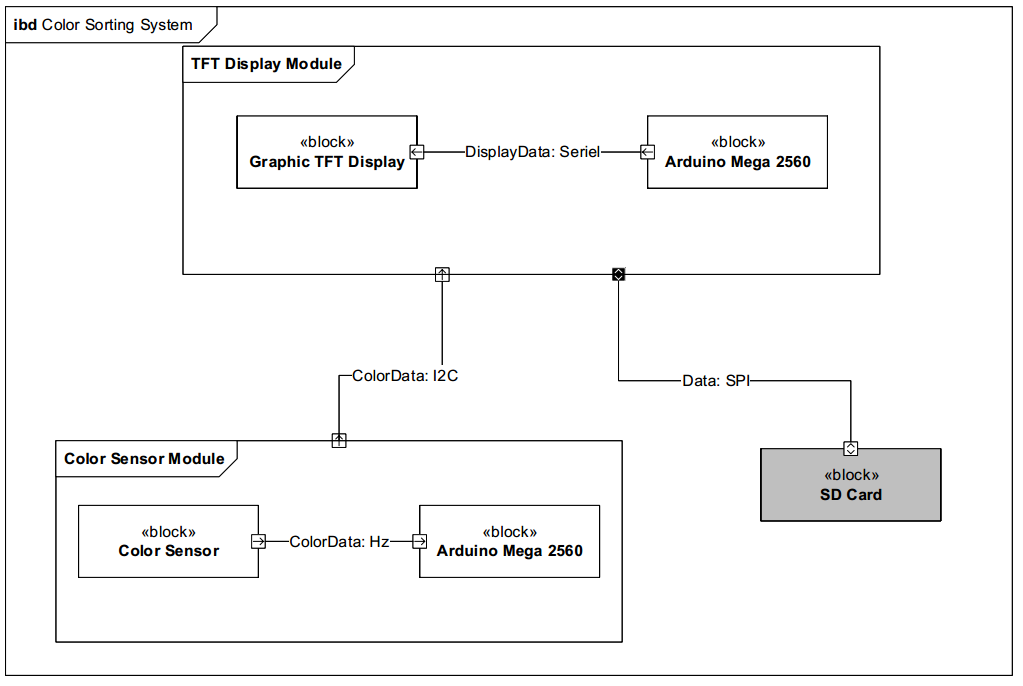
\includegraphics[width = 500pt]{Img/ColorSortingSystem_IBD.png}
	\caption{Color Sorting System IBD}
	\label{fig:ColorSortingSystem_IBD}
\end{figure}
%!TEX root = ../../Main.tex
\graphicspath{{Chapters/Teori/}}
%-------------------------------------------------------------------------------


\section{Color Sensor Module}
Color sensor modulet indeholder både en microcontroller og en color sensor. Til dette projekt har gruppen valgt at bruge en LC Technology TCS3200. Sensoren blev valgt fordi den var på lager i Embedded Stock, og at den ville passe godt til dette projekt. Til at styre denne sensor bruges en Arduino mega 2560.

\subsection{LC Technology TCS3200}
LC Technology TCS3200, virker ved at have 8x8 array af fotodioder. 16 fotodioder med et grønt filter, 16 fotodioder med et blåt filter, 16 fotodioder med et rødt filter og 16 fotodioder uden noget filter. De kan alle styres ved at sætte to pins(S2 og S3) høj eller lav. Se \autoref{fig:PinSelect}

\begin{figure}[H]
	\centering
	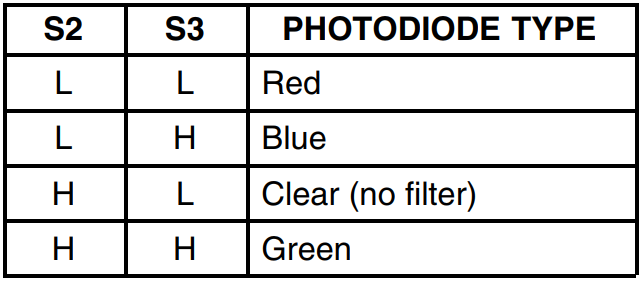
\includegraphics[width = 200pt]{Img/S1S2_color.png}
	\caption{Styring af photodioder}
	\label{fig:PinSelect}
\end{figure}

For at aflæse farveintensiteten, bliver man nødt til at måle på sensorens output pin. Signalet der kommer ud er et firkantssignal og farveintensiteten er bestemt alt efter hvor høj frekvensen er. For at se hvilken farve emnet har, bliver man nødt til at aktivere de forskellige fotodioder hver for sig, og tage en måling på output pin'en hver gang man har skiftet fotodiode. Derefter kan man så sammenligne de tre målinger (Clear bliver ikke målt) og se hvilket er størst. Hvis der skal måles andre farver end rød, grøn og blå, som fx gul, bliver man nødt til at kigge både på grøn og på rød. Hvis begge er lige høje må det være gul. Dog reagerer de forskellige fotodioder forskelligt på hvilken farve man ser på, så der skal der tages højde for. På \autoref{fig:FarveSpektrum} kan man se hvordan de forskellige fotodioder reagerer ved forskellige bølgelændger(farver).

\begin{figure}[H]
	\centering
	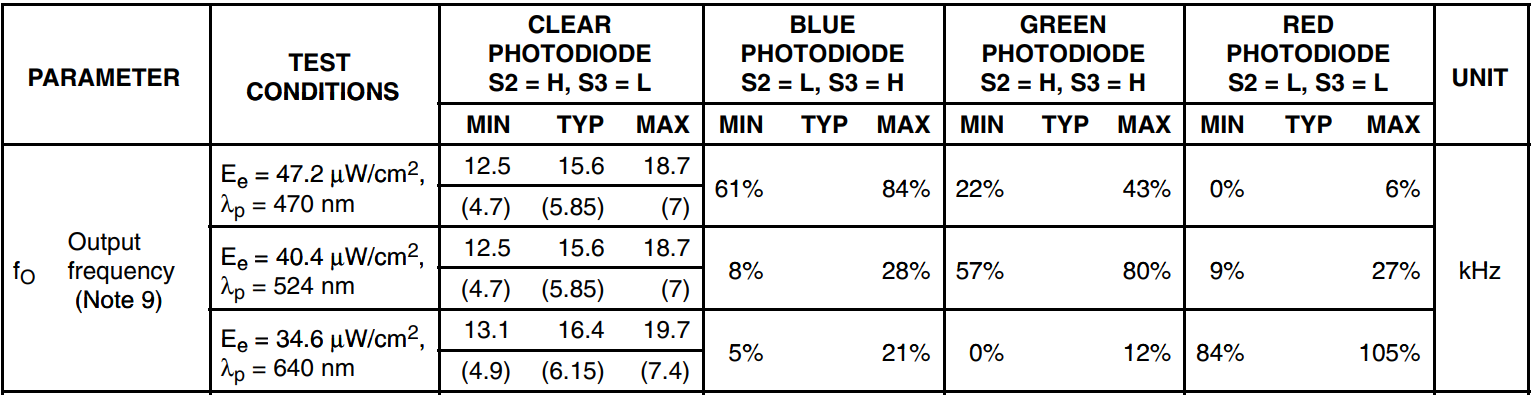
\includegraphics[width = 500pt]{Img/FarveSpektrum.png}
	\caption{Output frekvens ved forskellige farver}
	\label{fig:FarveSpektrum}
\end{figure}

En sidste ting der er værd er at vide om TCS3200, er dens indbygget frequency scaler. Den kan bruges til at styre skaleringen af output signalets frekvens. Skaleringen kan styres ved at sætte S1 og S2 høj eller lav. Til CSS bruges 2\% skalering, da 100\% skalering, ville betyde at output frekvensen kunne komme op over 50kHz. En lavere frekvens vil være fordelagtig i forhold til at få en præcis måling. Se \autoref{fig:Frekvens}

\begin{figure}[H]
	\centering
	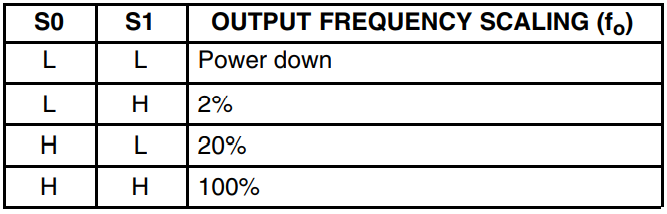
\includegraphics[width = 300pt]{Img/Frekvens.png}
	\caption{Output frekvens skalering}
	\label{fig:Frekvens}
\end{figure}

\subsection{Input Capture}
Input Capture er en metode der ofte bruges i embedded systemer, til at måle på diverse signaler. Til at måle outputsignalet fra TC3200 color sensor bruges denne metode.

\begin{figure}[H]
	\centering
	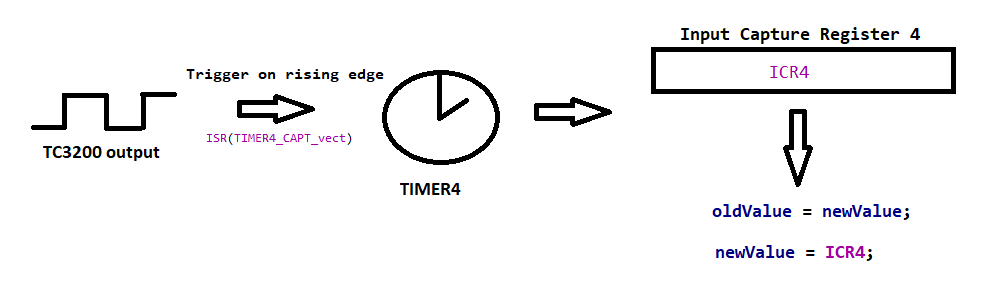
\includegraphics[width = 500pt]{Img/InputCapture.png}
	\caption{Input Capture illustration}
	\label{fig:InputCapture}
\end{figure}


Input Capture fungerer ved at have et interrupt der trigger på rising edge. Når dette interrupt bliver kaldt, tages et øjebliksbillede af TIMER4s værdi, som gemmes i Input Capture Register 4. Denne værdi gemmes i en variabel, som bagefter bruges til at beregne en frekvens. 

Derudover skal der også tages højde for overflow, ellers kan man risikerer at en måling ikke vil give en korrekt frekvens. For at udbedre dette problem bruges en anden interrupt, ISR(TIMER4\_OVF\_vect). Den trigger hver gang der kommer overflow, og 65535 lægges til newValue. Koden til hvordan frekvensen udregnes kan ses nedenunder.

\newpage
\begin{lstlisting}
ISR(TIMER4_CAPT_vect)
{
	oldValue = newValue;
	newValue = ICR4;
	
	if(newValue < oldValue)
	{
		period = oldValue-newValue;
	}
	else
	{
		newValue + overflow;
		period = oldValue - newValue;
	}
	freq = F_CPU/period;
	FREQFLAG = 1;
}

\end{lstlisting}

Det kan også ses i koden, hvordan overflow værdien lægges til newValue, hvis newValue er mindre end oldValue. FREQFLAG bruges så man altid er sikker på at freq har en ny værdi. FREQFLAG skal selvfølgelig sættes til 0, når man har brugt freq.

\subsection{Color Sensor Module Software}
For nemt at kunne forstå softwaren brugt til TC3200, er der blevet udarbejdet et data flow diagram, der giver et overblik over dataflowet i softwaren. Dette diagram kan ses på \autoref{fig:DataFlow}. Som det ses i diagrammet, bliver der taget en frekvensmåling for hver farve. Dette gøres, som beskrevet tidligere, ved at sætte S2 og S3 enten høj eller lav. Når en måling er taget, sammenlignes de tre målinger for at se hvilken farve er mest repræsenteret. Derefter sendes en char som enten er 'R', 'G' eller 'B'. Kommunikationen sker via I2C. Derefter starter koden forfra igen, og tager en ny frekvensmåling.

\begin{figure}[H]
	\centering
	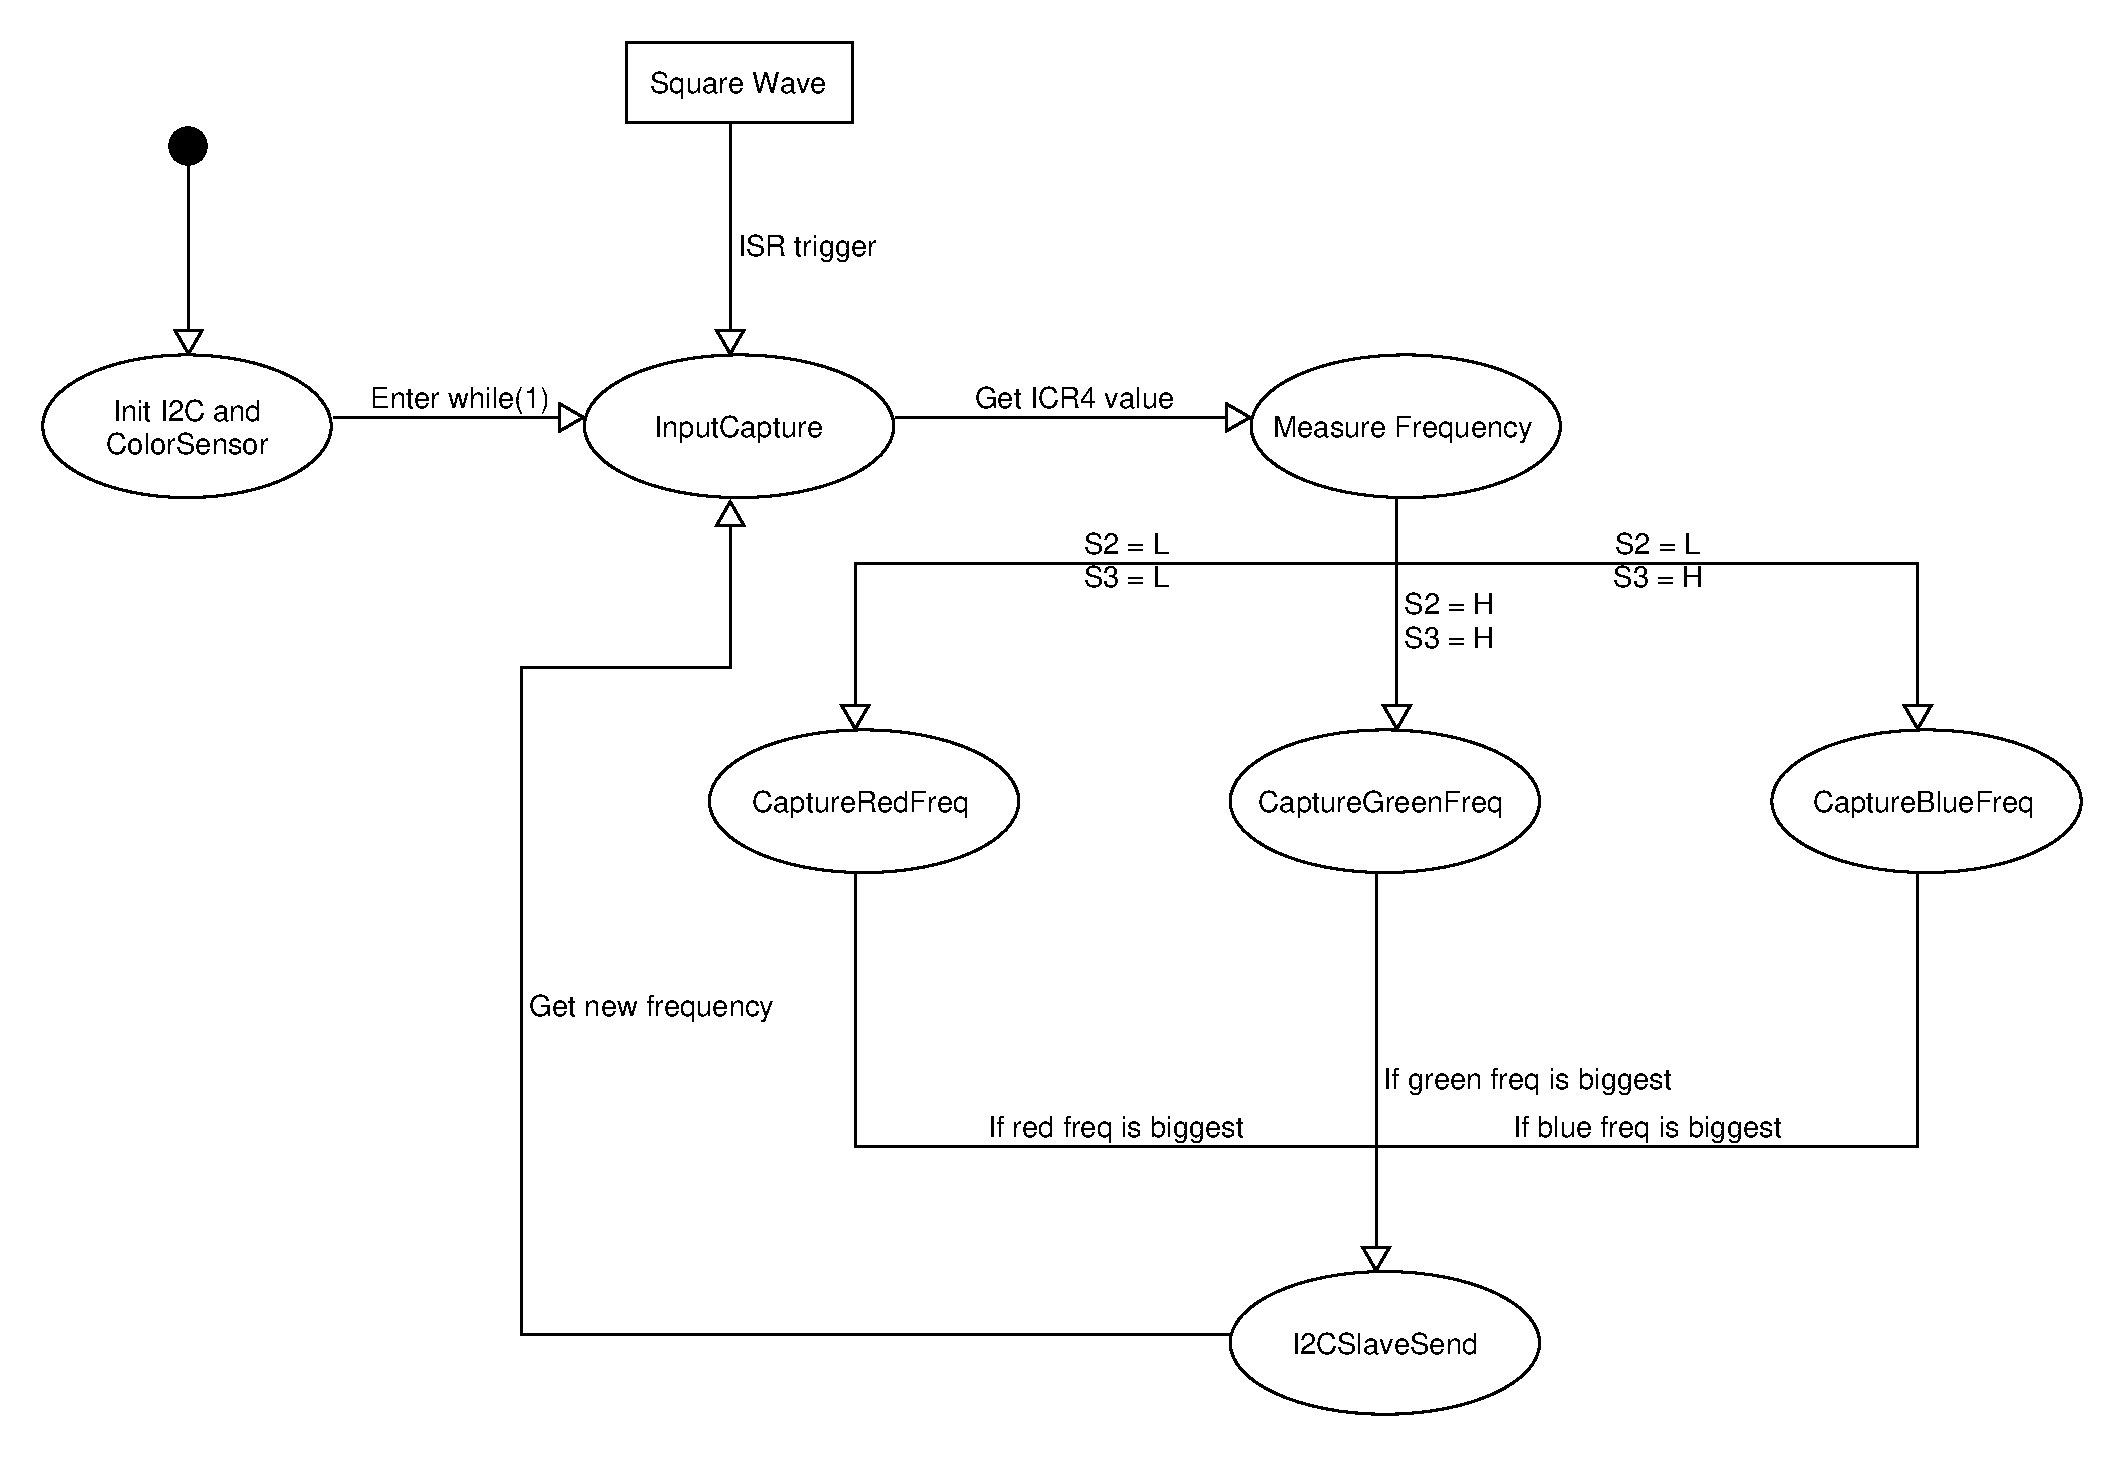
\includegraphics[width = 500pt]{Img/DataFlowDiagram.pdf}
	\caption{Data flow diagram}
	\label{fig:DataFlow}
\end{figure}

%!TEX root = ../../Main.tex
\graphicspath{{Chapters/Struktur/}}
%-------------------------------------------------------------------------------

\section{TFT Display Module}
TFT Display modulets primære opgave er både at fungere som visuel grænse flade til brugeren, samt at fungere som et slags kontrol modul for hele systemet. Kontrol modul forstået på den måde, at dette modul står for at hente data fra Color Sensor Modulet, og optælle den hentede information. Dette modul afsnit vil beskrive TFT Display modulets funktionalitet, samt overvejelser omkring analyse og design både hardware, softwaremæssigt. I dette afsnit vil kommunikationen mellem TFT Display modulet og resten af systemet også blive beskrevet. 

\subsection{Hardware}
I arkitekturfasen gik den første overvejelse på hvilket display vi skulle benytte som grænsefladen til brugeren. Vi ønskede et displayet som kunne vise farver og havde en nogenlunde opløsning for give en god visuel oplevelse for brugeren. Da vi først havde opsat kravene for vores display, var selve valget ikke særligt svært. I undervisningen har vi arbejdet med ”Graphic TFT Display”, dette display opfyldte vores ønskede krav angående opløsning samt muligheden for at vise farver. Derfor faldt valgt ret hurtigt på dette display, da det også spillede sammen med vores Arduino 2560. For at kunne påmontere ”Graphic TFT Display” på Arduino Mega 2560, har vi benyttet os af ”ITDB02 Arduino MEGA shield 2.0”. Databladet for dette shield er vedhæftet XX. I dette datablad er det også markeret hvilke porte ITDB02 shieldet der hører til bestemte indgange på displayet.

\subsection{Software}
I og med at dette moduls primære opgave er at være visuel grænseflade for brugeren, har langt det meste arbejde med dette modul lagt i softwaren. 
Hvis man kigger på Graphic TFT Display, kan den fungere i fire forskellige MCU-Interface modes, hvilket simpelt betyder, hvor stor en bus-interface man ønsker at arbejde med. Vi har valgt at arbejde med 16-bit bus-interface. 

\begin{figure}[H]
	\centering
	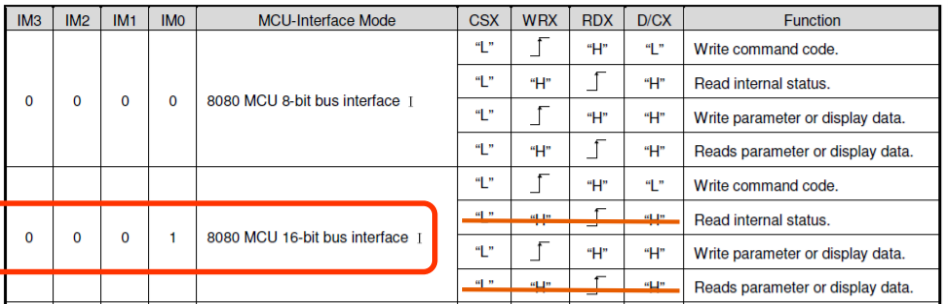
\includegraphics[width = 400pt]{Img/MCU-Interface_Mode.png}
	\caption{MCU-Interface Mode}
	\label{fig:MCU-Interface_Mode}
\end{figure}

I og med at vi udelukkende ønsker at skrive til vores display, vælger vi at ignorere læse kommandoerne og udelukkende fokusere på at skrive kommandoerne. Derfor er RDX altid sat høj.
Først implementerede vi WriteCommand i vores kode som ses på figur \autoref{fig:WriteCommand_Code} nedenfor

\begin{figure}[H]
	\centering
	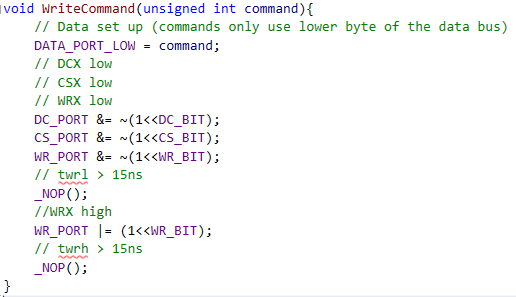
\includegraphics[width = 300pt]{Img/WriteCommand_Code.png}
	\caption{WriteCommand kode}
	\label{fig:WriteCommand_Code}
\end{figure}


Som det ses på figur \autoref{fig:MCU-Interface_Mode} fra databadet skal DCX og CSX sættes lavt, samt trigger kommandoen på WRX stigende flanke, derfor sættes WRX lav til at starte med. På figur \autoref{fig:Timedelays} nedenfor ses et skema over de tidsforsinkelser der opstår, ved forskellige operationer. Her ses det at når WRX sættes lav, opstår der en forsinkelse på min 15ns. Derfor er der indsat en NOP() funktion i koden, hvilket står for ”No Operation” som vil sige at programmet laver ingenting i en cyklus. Med en MCPU frekvens på 16Mhz svare det til 62,5ns. Herefter sættes WRX høj igen for at trigger kommandoen efterfulgt af endnu en NOP() funktion da der opstår samme forsinkelse når WRX sættes høj.

\begin{figure}[H]
	\centering
	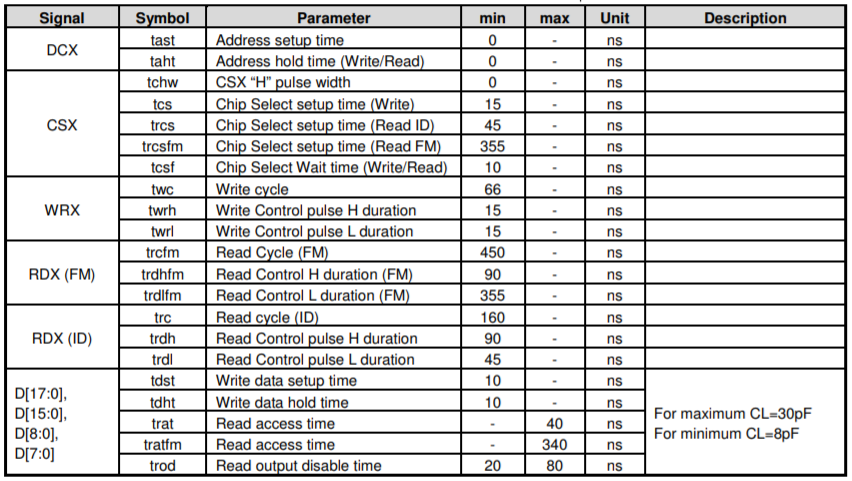
\includegraphics[width = 450pt]{Img/Timedelays.png}
	\caption{Tidsforsinkelser}
	\label{fig:Timedelays}
\end{figure}


Dernæst implementerede vi WriteData, som tilnærmelsesvis ligner WriteCommand bortset fra at DCX skal sættes høj i stedet for lav. Koden for WriteData ses nedenfor på figur \autoref{fig:WriteData_Code}. På samme måde som WriteCommand trigger WriteData på en voksende flanke på WRX, derfor sættes WRX først lav og dernæst høj, med indsat NOP() funktioner for at tage højde for tidsforsinkelser. 

\begin{figure}[H]
	\centering
	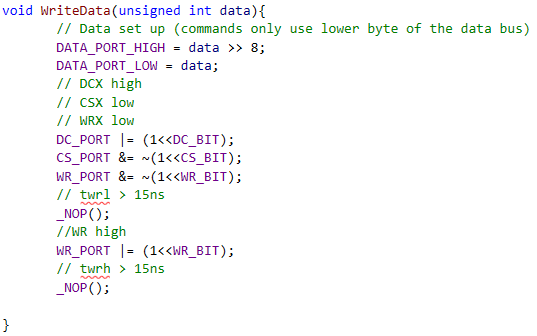
\includegraphics[width = 350pt]{Img/WriteData_Code.png}
	\caption{WriteData kode}
	\label{fig:WriteData_Code}
\end{figure}


I vores DisplayInit() som vi kalder en gang i koden til at Initialisere displayet, starter vi med at sætte vores Control Pins som outputs, samt sætte dem høje. Dernæst bliver RST sat lav i 300ms, det skyldes at der i databladet på side 230 står minimum 120ms, så det er sat til 300ms for at være på den sikre side. Efter vi igen sætter RST igen bliver sat høj, skal vi igen vente 120ms før vi må kalde SleepOut Command, derfor indsætter et delay på 130ms. Herefter vækkes displayet med Sleepout() kommandoen efterfulgt af Displayon(). Begge disse kommandoer er at finde i databladet på side 83. Den kommando der bliver sendt til MemoryAccessControl() sørger for at sætte rækkefølgen til BGR i stedet for RGB. Til sidst bliver en kommando sendt til InterfacePixelFormat(), denne kommando fortæller displayet at vi ønsker at køre med 16bit pr. pixel se side 134 i databladet. 

\begin{figure}[H]
	\centering
	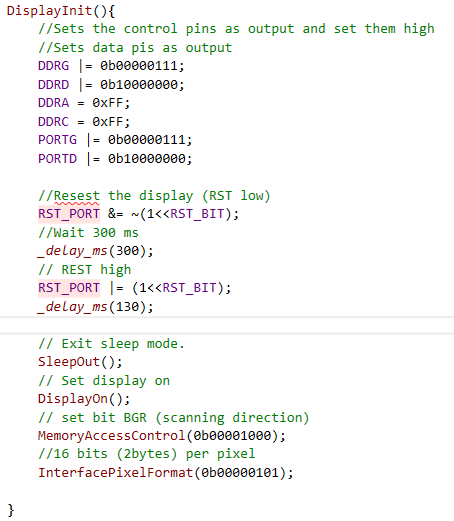
\includegraphics[width = 300pt]{Img/DisplayInit_Code.png}
	\caption{DisplayInit kode}
	\label{fig:DisplayInit_Code}
\end{figure}


Efter at have initialiseret og opsat displayet efter egen ønske. Var den næste opgave at kunne skrive tal og bogstaver ud på vores display. Til dette benyttede vi os af et program ved navn ’TheDotFactory’. Vi fik programmet til at udskrive et kæmpe array, som indeholder alle symboler, tal samt bogstaver vi kunne havde brug for. Sammen med et tilhørende array, der fortæller længden af hvert symbol samt dens offset. Disse to arrays genereret af programmet ’TheDotFactory’ har vi lagt ind i en h-fil ved navn ”DotFactory.h”.
På den efterfølgende \autoref{TFTDisplayFunktioner} vil funktionerne vi har benyttet blive overordnet blive beskrevet, i vores vedlagte kode vil en mere detaljeret gennemgang af koden kunne ses, i form af kommentar til hver linje kode i den vedlagte kode. 

\newpage

\begin{table}[]
	\centering
	\caption{Funktioner benyttet til TFT Display}
	\label{TFTDisplayFunktioner}
	\begin{tabular}{|l|l|}
		\hline
		\textbf{Navn}         & \textbf{Beskrivelse}                                                                                                                                                              \\ \hline
		WritePixel() & \begin{tabular}[c]{@{}l@{}}Formået er at bestemme farven for en pixel. Tager imod 3 parameter.\\ Rød 0-31, grøn 0-63, blå 0-31 smider dem ind i write data.\end{tabular} \\ \hline
		SetColomnAddress() & \begin{tabular}[c]{@{}l@{}}Formålet er at kunne skrive til en hel linje lodret på en gang.\\ Tager imod to parameter start og stop.\end{tabular}                                                                                                                                                                         \\ \hline
		SetPageAddress() & \begin{tabular}[c]{@{}l@{}} Formålet er at kunne skrive til en hel linje vandret på en gang.\\ Tager imod to parameter start og stop. \end{tabular}                                                                                                                                                                        \\ \hline
		FillRectangle() & \begin{tabular}[c]{@{}l@{}} Meningen er at fylde et rektangel med én farve.\\ Tager imod syv parametre: start-x, start-y, bredde, højde,\\ rød, blå og grøn.  \end{tabular}  \\ \hline
		getSymbolParameters() &  \begin{tabular}[c]{@{}l@{}} Den tager tre parametre, start x og start y samt længden på det\\ givne symbol. Formået for denne funktion er at opdele alle de\\ nødvendige informationer for et symbol. Så som længen af symbolet\\ i byte, offset i forhold til arrayet fra TheDotFactory, offset i forhold\\ til displayet. Denne information bliver så videregivet til drawSymbol(). \end{tabular}   \\ \hline
		drawSymbol() &  \begin{tabular}[c]{@{}l@{}}Tager information videregivet fra getSymbolParameters(). Finder det\\ givne symbol i arrayet fra TheDotFactory ved hjælp af informationen.\\ Herefter gennemgås symbolet bit for bit, og displayet\\ en sort pixel eller hvid pixel alt efter om det er et ’1’ eller ’0’\\ på den givne plads.  \end{tabular}                                                                                                                                                                                         \\ \hline
		writeString() & \begin{tabular}[c]{@{}l@{}} Tager imod en string. Hvorefter den gennemgår denne string symbol\\ for symbol og kalder getSymbolParameters () som videre kalder\\ drawSymbol() på hvert symbol. Med mindre at symbolet er et\\ mellemrum, så plusses x-positionen med seks.  \end{tabular}                                                                                                                                                                                         \\ \hline
		writeInt() &  \begin{tabular}[c]{@{}l@{}} Tager imod en long int. Hvorefter den int bliver lagt over i et array.\\ Og på hver plads i dette array bliver getSymbolParameters kaldt,\\ efter det første tal er detekteret.   \end{tabular}                                                                                                                                                                                         \\ \hline
		\begin{tabular}[c]{@{}l@{}} DrawRed(),\\ DrawGreen(),\\ DrawBlue() \end{tabular}  &  \begin{tabular}[c]{@{}l@{}} Meningen med denne funktion er at vise en søjle i enten farven rød,\\ grøn eller blå alt efter hvilken af disse tre funktioner der bliver kaldt.\\ Over denne søjle skal så skrives et tal, som følger søjlens højde.\\ Funktionerne modtager to int, den første int angiver tallet som skal\\ stå over søjlen, den anden int angiver højden på søjlen. Tallet\\ bliver vist ved hjælp af funktionen writeInt(), og søjlen bliver vist ved\\ hjælp af funktionen FillRectangle(). Den eneste forskel på disse tre\\ funktioner er farven af søjlen.  \end{tabular} \\ \hline
		drawTotal() &  \begin{tabular}[c]{@{}l@{}} Meningen med denne funktion er at den skal tage tre parametre som\\ antallet af hver farve detekteret. Disse tre parametre bliver så lagt\\ sammen i en totalCount variable, og udregnet hvor stor en procentdel\\ de hver udgør at det samlet antal optællinger. Den procentdel\\ udgør så hvor høj hver enkel søjle skal være. Så vil DrawRed(),\\ DrawGreen() og DrawBlue() blive kaldt hvor de tre parametre vil\\ være tallene over søjlerne, højden vil være den udregnede\\ procentdel og totalCount vil blive vist i øverste højre hjørne\\ ved hjælp af writeInt().  \end{tabular}                                                                                                                                                                                         \\ \hline
	\end{tabular}
\end{table}
%!TEX root = ../../Main.tex
\graphicspath{{Chapters/Matlab/}}
%-------------------------------------------------------------------------------







%!TEX root = ../../Main.tex
\graphicspath{{Chapters/Test/}}
%-------------------------------------------------------------------------------


\section{I2C kommunikation}
Til at starte med havde gruppen ikke planer om at inkorporere I2C i NSS, da den simple løsning var at have både TFT skærmen og Color Sensoren sat til samme Arduino. Dette viste sig ikke at kunne lade sig gøre, da skærmen og sensoren delte nogle pins, hvilket gjorde at systemet ikke fungerede. Desværre kunne vi ikke bruge andre pins til sensoren, da de to pins der er at vælge imellem begge sad i vejen for skærmen. Derfor valgte gruppen at splitte systemet op og anvende I2C. På grund af denne ekstra arbejsbyrde, blev SD kort implementationen nedprioriteret.



\subsection{I2C master}
Masteren blev valgt implementeret på TFT display modulet, da det ikke ville give mening at lade sensor modulet sende kommandoer til display modulet. Istedet for sendes der en char fra slaven, som repræsenterer en farve.

Før masteren kan bruges skal den først initiereres. Dette sker ved at sætte bestemte dataregistre op rigtigt. Først bestemmer man hvilken clock SCL skal have. SCL kan udregens på følgende måde:

\begin{equation}
SCL= \frac{CPU}{16+2(TWBR)*4^{TWPS}} 
\end{equation}

Gruppen har valgt at en clock på 500KHz. De eneste krav til clokcen er at den er 16 gange lavere end slavens cpu clock, ifølge megea 2560 datablad. Da slaven kører med 16MHz, opfylder den det krav. 



\begin{figure}[H]
	\centering
	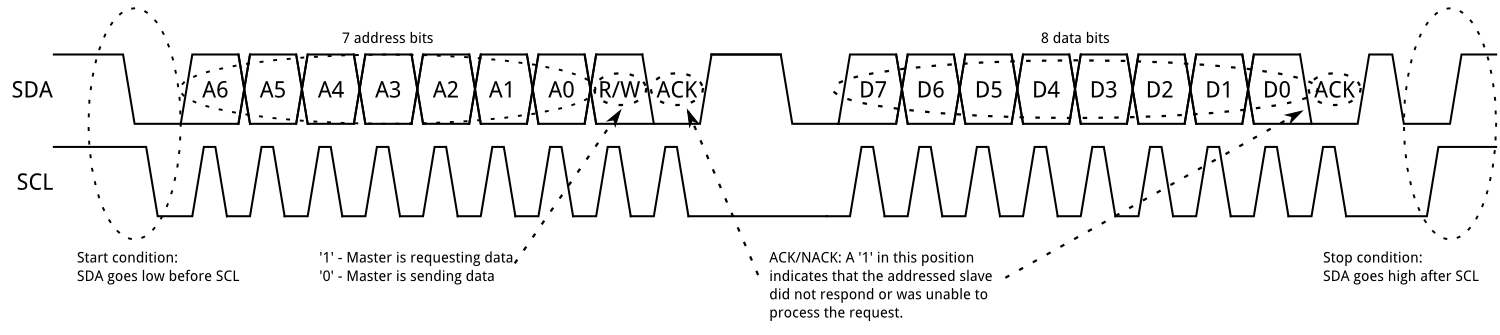
\includegraphics[width = 450pt]{Img/I2CTiming.png}
	\caption{I2C timing diagram}
	\label{fig:I2CTIming}
\end{figure}


Til udviklingen af masteren har et timing diagram over I2C protokollen, se \autoref{fig:I2CTIming}, været utrolig nyttig. Ved hjælp af dette diagram har gruppen kunne sende korrekte beskeder over I2C. 

For at have en så overskuelig kode som overhovedet muligt, er der blevet lavet funktioner der kan generere ACK, NACK, WAIT, START og STOP. Disse funktioner er så brugt i vores i2c\_master\_receive funktion. Et Kodeudsnit af denne funktion kan findes nedenunder:

\newpage

\begin{lstlisting}
i2c_master_start();
while(transfer && i < 250)
{
	//usart_transmit(twi_master_status());
	switch (i2c_master_status())
	{
		// Start condition has been transmitted
		case 0x08:
		// Contact slave and enter master transmitter mode
		TWDR = address_r;
		i2c_master_ack();
		i2c_master_wait();
		break;
		
		// SLA+R has been transmitted and acked
		case 0x40:
		i2c_master_nack();
		i2c_master_wait();
		break;
		
		// Data byte has been received and acked
		case 0x50:
		//SendChar('A');
		data = TWDR;
		transfer = 0;
		break;
		
		// Data byte has been received and nacked
		case 0x58:
		//SendChar('B');
		data = TWDR;
		transfer = 0;
		break;
	}
	i++;
}
i2c_master_stop();
\end{lstlisting}

Som det ses i koden bliver i2c\_master\_status() hele tiden tjekket på, for at finde ud af om slaven reagerer på nogle af kommandoerne fra masteren. Status funktion tjekker TWSR registeret og AND'er det med 0xF8, for at sætte de tre sidste bits til 0. I mega 2560 datablad kan der findes en tabel over hvad de forskellige status koder står for. I kode udsnittet står de som kommentarer over hver case.

\subsection{I2C slave}
Ligesom masteren skal slave også initialiseres, ved at sætte nogle bestemte dataregistre op. TWAR registeret bestemmer slavens adresse, i vores tilfælde er den sat til 40. TWCR registeret bestemmer hvilken slave mode den skal sættes i, i vores tilfælde er det slave transmitter mode. Det vil sige at slaven kun skal kunne sende data til masteren, og ikke omvendt. 

Når slaven er sat op i transmitter mode, bliver der gjort brug af et interrupt, der når i2c interfacet bliver brugt. Når et interrupt bliver triggered, køres vores interrupt rutine, som kan ses nedenunder:

\begin{lstlisting}
if(i2c_slave_addressed())
{
	
	switch(i2c_slave_status())
	{
		
		case 0x60:
		i2c_slave_ack();
		break;
		
		case 0x80:
		SendChar('A');
		data = TWDR;
		i2c_slave_ack();
		transfering = 0;
		break;
		
		case 0xA8:
		TWDR = dataToSend; //data send to master
		i2c_slave_ack();
		break;
		
		// Last byte sent by master
		case 0xC0:
		transfering = 0;
		i2c_slave_ack();
		break;
	}
}
\end{lstlisting}

Interrupt rutinen minder meget om masterens receive funktion. Den tjekker hele tiden på status registeret(TWSR), for at holde styr på hvor langt den er i I2C processen. dataToSend indeholder en char med information om hvilken farve color sensoren har opfanget. 



\subsection{Test}

Til test af I2C, har vi gjort brug af en logic analyzer, som bruges til at afkode beskeder der sende med forskellige protokoller. Det har været en stor hjælp til at finde fejl i vores software. Blandt andet fandt vi ud af at hvis UART og I2C blev brugt samtidig, skabte det en stor nok forsinkelse i I2C protokollen. Dette skyldes at der ikke blev sendt et ACK på det rigtige tidspunkt. 

\begin{figure}[H]
	\centering
	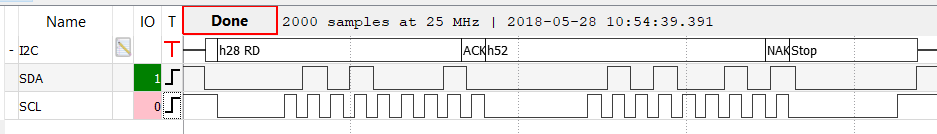
\includegraphics[width = 450pt]{Img/I2C_logic.png}
	\caption{Logic analyzer for I2C}
	\label{fig:I2C_Logic}
\end{figure}

På figuren ovenfor kan man se en perfekt I2C transmission. På figuren kan man se at et start condition, starter transmissionen, hvorefter adressen på slaven bliver sendt og at R/Wbit bliver sat højt, hvilket betyder READ. Derfter kommer dataen. I dette tilfælde bliver der sendt h52, hvilket svarer i ASCII svarer til bogstavet 'R'. Et NACK kommer bagefter for at signallere at der ikke er mere data, hvorefter et stop condition blever genereret.


%!TEX root = ../../Main.tex
\graphicspath{{Chapters/Alternative_Loesninger/}}
%-------------------------------------------------------------------------------


\section{Alternative Løsninger}
I dette afsnit vil fordele og ulemper for forskellige alternative løsninger blive diskuteret.


\subsection{Valg af Kommunikation}


\subsection{Valg af color sensor}


\subsection{Valg af skærm}
\include{Chapters/CSS_test/Css_test}
%!TEX root = ../../Main.tex
\graphicspath{{Chapters/Konklussion/}}
%-------------------------------------------------------------------------------


\section{Konklussion}
Der er i dette AMS-projekt blevet udviklet et farve sorterings system, ved navn Color Sorting System. Systemet kan genkende tre forskellige farver - rød, grøn og blå. Et objekt med en af disse tre farver placeres under systemet, og ved hjælp af brugerinteraktion i from af en knap, bestemmer brugeren hvornår farvebestemmelsen skal udføres. Et display fungerer som grænseflade til brugeren, hvorpå tre søjler med farverne rød, grøn og blå vil vises. Søjlerne vil have individuel højde relativ til antal målinger af pågældende farve.  \\\\
Grundet tidsmangel og udfordringer har ideen med produktet ændret sig undervejs. Det glæder både nedprioriteringer, som meget af det mekaniske er blevet grundet tidsmangel. Samt ændringer af projektet grundet udfordringer, der gjorde at gruppen prioriterede I2C kommunikation frem for SPI kommunikation med SD kort. \\\\
Under AMS-projekt forløbet har gruppen gjort brug af teori fra undervisningen, samt tilegnet sig ny information til at udvikle på produktet. \\\\
Alt i alt er gruppen godt tilfreds med det endelige produkt, selvom produktideen grundet problemer ændrede sig et par gange undervejs. Gjorde det bare at vi som gruppe har skulle finde på nye løsninger, som har gjort forløbet både udfordrende og lærerigt på samme tid.


\begin{flushleft}
	
\end{flushleft}


\bibliographystyle{plain}
\bibliography{Bibliography}	

 
\end{document}